% ============================================================
%  MindMonitor — Technical Architecture Report
%  Author: MDTAHSINURRAHMAN  |  April 2026
% ============================================================
\documentclass[12pt,a4paper]{report}

\usepackage[margin=2.5cm]{geometry}
\usepackage[T1]{fontenc}
\usepackage[utf8]{inputenc}
\usepackage{lmodern}
\usepackage{microtype}
\usepackage{hyperref}
\usepackage{xcolor}
\usepackage{graphicx}
\usepackage{tikz}
\usetikzlibrary{shapes.geometric,arrows.meta,positioning,fit,backgrounds,calc}
\usepackage{listings}
\usepackage{booktabs}
\usepackage{tabularx}
\usepackage{multirow}
\usepackage{fancyhdr}
\usepackage{titlesec}
\usepackage{enumitem}
\usepackage{tcolorbox}
\tcbuselibrary{skins,breakable}
\usepackage{float}
\usepackage{caption}

% ── Colours ─────────────────────────────────────────────────
\definecolor{primary}{HTML}{7C3AED}
\definecolor{secondary}{HTML}{0EA5E9}
\definecolor{accent}{HTML}{F43F5E}
\definecolor{dark}{HTML}{1F2937}
\definecolor{midgray}{HTML}{6B7280}
\definecolor{lightgray}{HTML}{F3F4F6}
\definecolor{codegreen}{HTML}{10B981}
\definecolor{codeblue}{HTML}{3B82F6}
\definecolor{success}{HTML}{059669}
\definecolor{warning}{HTML}{D97706}
\definecolor{danger}{HTML}{DC2626}
\definecolor{codeyellow}{HTML}{F59E0B}

\hypersetup{colorlinks=true,linkcolor=primary,urlcolor=secondary,
  pdftitle={MindMonitor Architecture Report},pdfauthor={MDTAHSINURRAHMAN}}

% ── Page style ──────────────────────────────────────────────
\pagestyle{fancy}\fancyhf{}
\fancyhead[L]{\textcolor{midgray}{\small MindMonitor — Architecture Report}}
\fancyhead[R]{\textcolor{midgray}{\small April 2026}}
\fancyfoot[C]{\thepage}
\renewcommand{\headrulewidth}{0.4pt}

\titleformat{\chapter}[display]
  {\normalfont\huge\bfseries\color{primary}}{\chaptertitlename\ \thechapter}{16pt}{\huge}
\titleformat{\section}{\normalfont\large\bfseries\color{dark}}{\thesection}{1em}{}
\titleformat{\subsection}{\normalfont\normalsize\bfseries\color{midgray}}{\thesubsection}{1em}{}

% ── Listings ────────────────────────────────────────────────
\lstset{
  backgroundcolor=\color{lightgray},
  commentstyle=\color{codegreen},
  keywordstyle=\color{primary},
  stringstyle=\color{codeblue},
  basicstyle=\ttfamily\footnotesize,
  breaklines=true, numbers=left, numberstyle=\tiny\color{midgray},
  numbersep=5pt, frame=single, rulecolor=\color{midgray!40},
  showstringspaces=false, tabsize=2
}

% ── Boxes ───────────────────────────────────────────────────
\newtcolorbox{infobox}[1][]{colback=secondary!8,colframe=secondary,
  fonttitle=\bfseries,title=#1,breakable}
\newtcolorbox{warnbox}[1][]{colback=warning!8,colframe=warning,
  fonttitle=\bfseries,title=#1,breakable}
\newtcolorbox{dangerbox}[1][]{colback=danger!8,colframe=danger,
  fonttitle=\bfseries,title=#1,breakable}
\newtcolorbox{techbox}[1][]{colback=primary!6,colframe=primary,
  fonttitle=\bfseries,title=#1,breakable}

% ── TikZ styles ─────────────────────────────────────────────
\tikzset{
  arr/.style={-{Stealth[length=5pt]},thick},
  darr/.style={<->,thick},
  box/.style={rectangle,rounded corners=4pt,minimum width=2.4cm,
    minimum height=0.75cm,text centered,font=\small\bfseries,draw,thick},
  dbox/.style={cylinder,shape border rotate=90,aspect=0.25,
    minimum width=2cm,minimum height=0.9cm,text centered,
    font=\small\bfseries,draw=midgray,fill=lightgray!60,thick},
  cbox/.style={ellipse,minimum width=2.4cm,minimum height=0.9cm,
    text centered,font=\small\bfseries,draw,thick},
  lyr/.style={rectangle,rounded corners=6pt,draw=midgray!50,
    dashed,thick,inner sep=10pt},
}

% ============================================================
\begin{document}

% ── Title Page ──────────────────────────────────────────────
\begin{titlepage}
\pagecolor{dark}\color{white}\centering\vspace*{2.5cm}
{\fontsize{40}{48}\selectfont\bfseries\color{primary}MindMonitor}\\[0.5cm]
{\LARGE\color{white!80}Mental Health Monitoring Platform}\\[1.5cm]
\textcolor{primary}{\rule{12cm}{2pt}}\\[0.3cm]
\textcolor{secondary}{\rule{12cm}{0.8pt}}\\[1.5cm]
{\Large\bfseries Comprehensive Technical Architecture Report}\\[0.4cm]
{\normalsize Authentication $\cdot$ Database $\cdot$ Firebase $\cdot$ Real-time Sync}\\
{\normalsize Video Calls $\cdot$ IoT Sensors $\cdot$ Anomaly Detection}\\[2.5cm]
\begin{tabular}{rl}
\textbf{Author:}    & MDTAHSINURRAHMAN \\[3pt]
\textbf{Email:}     & mahmud2007068@stud.kuet.ac.bd \\[3pt]
\textbf{Date:}      & April 2026 \\[3pt]
\textbf{Framework:} & Next.js 16 / TypeScript / Supabase / Firebase \\
\end{tabular}
\vfill
{\small\color{white!50}KUET --- Khulna University of Engineering \& Technology}
\end{titlepage}
\pagecolor{white}\color{black}

\chapter*{Abstract}\addcontentsline{toc}{chapter}{Abstract}
MindMonitor is a full-stack web platform for continuous physiological and mental health monitoring. It connects Arduino/ESP8266 hardware sensors to a React web interface via a dual-database architecture: \textbf{Firebase Realtime Database} for sub-second live streaming and \textbf{PostgreSQL} (via Supabase) for persistent clinical records. Authentication uses Supabase Auth (JWT in HTTP-only cookies). Role-based access control separates patients from doctors. Video consultations are powered by ZegoCloud. This report documents every architectural component, their interconnections, and the complete data flow.

\tableofcontents
\clearpage

% ============================================================
\chapter{System Overview}

\section{Technology Stack}

\begin{table}[H]\centering\renewcommand{\arraystretch}{1.4}
\begin{tabularx}{\linewidth}{>{\bfseries}l l X}
\toprule
Layer & Technology & Purpose \\
\midrule
Frontend & Next.js 16.1.6 + React 19 & App Router, SSR, API routes, middleware \\
Styling & Tailwind CSS v4 + Framer Motion 12 & Utility CSS, animations \\
Charts & Recharts 3.7 & Sensor data visualizations \\
\midrule
Auth & Supabase Auth + @supabase/ssr & JWT cookie sessions, SSR validation \\
\midrule
Primary DB & PostgreSQL (Supabase hosted) & Persistent relational storage \\
ORM & Prisma 6.19 & Type-safe queries and migrations \\
Realtime DB & Firebase RTDB 12 & Sub-second sensor streaming \\
\midrule
Video & ZegoCloud UIKit Prebuilt 2.17 & WebRTC video call rooms \\
Validation & Zod 4.3 & Runtime schema validation \\
Hardware & Arduino / ESP8266 & Sensor acquisition (GSR, HR, SpO2, Temp) \\
\bottomrule
\end{tabularx}
\caption{Complete technology stack}
\end{table}

\section{High-Level Architecture}

\begin{figure}[H]\centering
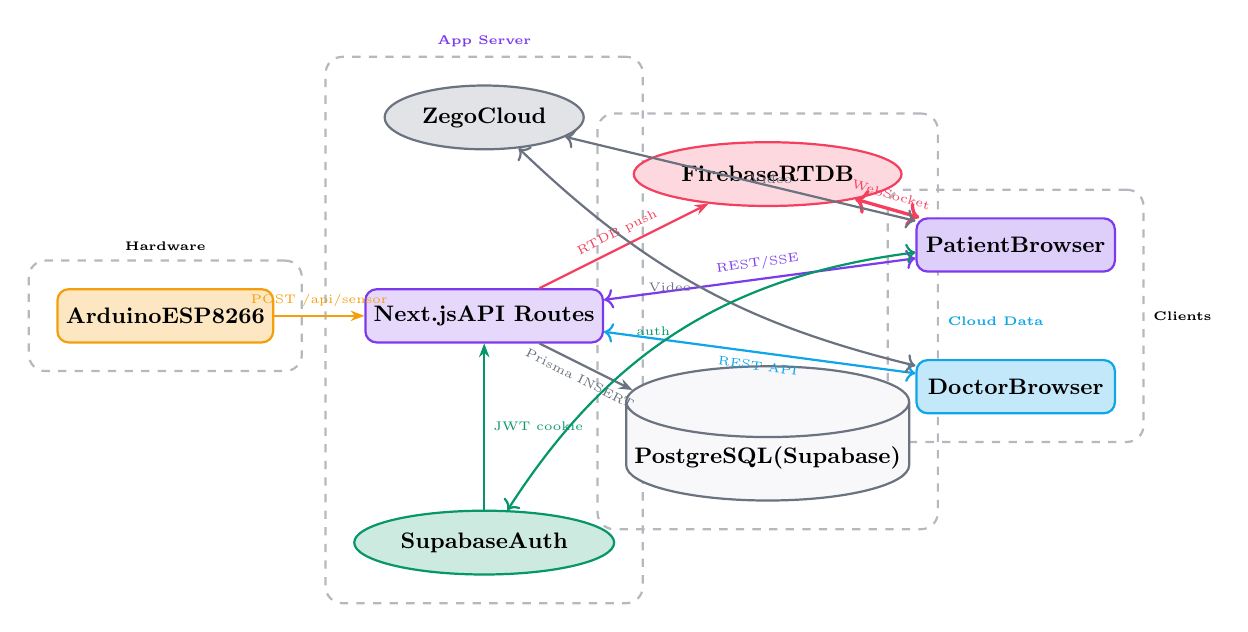
\begin{tikzpicture}[node distance=1.5cm,scale=0.9,transform shape]

\node[box,fill=codeyellow!25,draw=codeyellow] (hw) at (0,0) {Arduino\\ESP8266};
\node[box,fill=primary!20,draw=primary] (api) at (4.5,0) {Next.js\\API Routes};
\node[cbox,fill=accent!20,draw=accent] (fb) at (8.5,2) {Firebase\\RTDB};
\node[dbox] (pg) at (8.5,-2) {PostgreSQL\\(Supabase)};
\node[cbox,fill=success!20,draw=success] (auth) at (4.5,-3.2) {Supabase\\Auth};
\node[cbox,fill=midgray!20,draw=midgray] (zego) at (4.5,2.8) {ZegoCloud};
\node[box,fill=primary!25,draw=primary,minimum width=2.8cm] (pat) at (12,1) {Patient\\Browser};
\node[box,fill=secondary!25,draw=secondary,minimum width=2.8cm] (doc) at (12,-1) {Doctor\\Browser};

\draw[arr,codeyellow] (hw) -- node[above,font=\tiny]{POST /api/sensor} (api);
\draw[arr,accent] (api) -- node[above,font=\tiny,sloped]{RTDB push} (fb);
\draw[arr,midgray] (api) -- node[below,font=\tiny,sloped]{Prisma INSERT} (pg);
\draw[arr,success] (auth) -- node[right,font=\tiny]{JWT cookie} (api);
\draw[darr,accent,very thick] (fb) -- node[above,font=\tiny,sloped]{WebSocket} (pat);
\draw[darr,primary] (api) -- node[above,font=\tiny,sloped]{REST/SSE} (pat);
\draw[darr,secondary] (api) -- node[below,font=\tiny,sloped]{REST API} (doc);
\draw[darr,midgray] (zego) -- node[right,font=\tiny]{Video} (pat);
\draw[darr,midgray] (zego) to[bend right=15] node[left,font=\tiny]{Video} (doc);
\draw[darr,success] (pat) to[bend right=25] node[left,font=\tiny]{auth} (auth);

\begin{scope}[on background layer]
  \node[lyr,fit=(hw),label={[font=\tiny\bfseries]above:Hardware}] {};
  \node[lyr,fit=(api)(auth)(zego),label={[font=\tiny\bfseries,primary]above:App Server}] {};
  \node[lyr,fit=(fb)(pg),label={[font=\tiny\bfseries,secondary]right:Cloud Data}] {};
  \node[lyr,fit=(pat)(doc),label={[font=\tiny\bfseries]right:Clients}] {};
\end{scope}
\end{tikzpicture}
\caption{High-level system architecture}
\end{figure}

% ============================================================
\chapter{Authentication and Sessions}

\section{How Sessions Work}

Authentication is delegated entirely to \textbf{Supabase Auth}. It issues \textbf{JWT (JSON Web Tokens)} stored in \textbf{HTTP-only cookies} --- not \texttt{localStorage} --- to enable server-side validation without JavaScript.

\begin{figure}[H]\centering
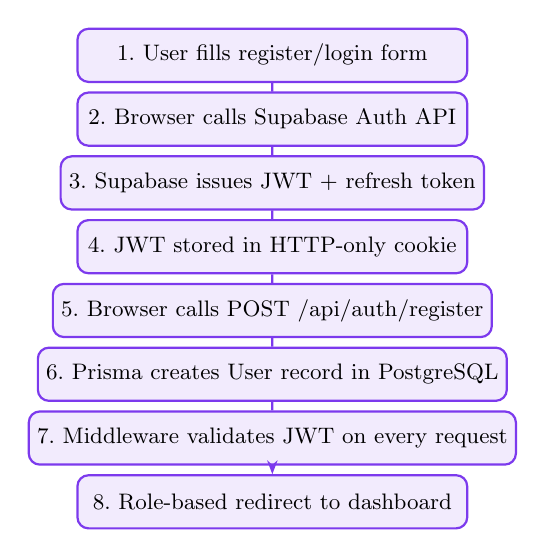
\begin{tikzpicture}[node distance=0.9cm,scale=0.9,transform shape,
  s/.style={box,fill=primary!10,draw=primary,minimum width=5.5cm,font=\small}]

\node[s] (r1) {1.\ User fills register/login form};
\node[s,below of=r1] (r2) {2.\ Browser calls Supabase Auth API};
\node[s,below of=r2] (r3) {3.\ Supabase issues JWT + refresh token};
\node[s,below of=r3] (r4) {4.\ JWT stored in HTTP-only cookie};
\node[s,below of=r4] (r5) {5.\ Browser calls POST /api/auth/register};
\node[s,below of=r5] (r6) {6.\ Prisma creates User record in PostgreSQL};
\node[s,below of=r6] (r7) {7.\ Middleware validates JWT on every request};
\node[s,below of=r7] (r8) {8.\ Role-based redirect to dashboard};

\draw[arr,primary] (r1)--(r2)--(r3)--(r4)--(r5)--(r6)--(r7)--(r8);
\end{tikzpicture}
\caption{Registration and session establishment flow}
\end{figure}

\textbf{Cookie properties:} HTTP-only (no JS access), SameSite=Lax (CSRF protection), Secure (HTTPS only), auto-refreshed by \texttt{@supabase/ssr} using the refresh token.

\section{Two Supabase Clients}

\begin{lstlisting}[language=TypeScript,caption={src/lib/supabase.ts}]
// Browser client — reads/writes cookies automatically
export const createBrowserClient = () =>
  createClient(SUPABASE_URL, SUPABASE_ANON_KEY);

// Admin client — service-role key, SERVER-SIDE ONLY
export const createAdminClient = () =>
  createClient(SUPABASE_URL, SUPABASE_SERVICE_ROLE_KEY);
\end{lstlisting}

\section{Middleware — Route Guards}

\textbf{File:} \texttt{src/middleware.ts} --- runs on every request before any page or API handler.

\begin{table}[H]\centering\renewcommand{\arraystretch}{1.4}
\begin{tabularx}{\linewidth}{>{\ttfamily\small}l l X}
\toprule
Path & Auth Required & Redirect Logic \\
\midrule
/doctor/dashboard/* & Yes (DOCTOR) & Unauthed $\to$ /login; Patient role $\to$ /patient/dashboard \\
/patient/dashboard/* & Yes (PATIENT) & Unauthed $\to$ /login; Doctor role $\to$ /doctor/dashboard \\
/login, /register & No & If already logged in $\to$ role dashboard \\
/api/sensor & Exempt & Hardware webhook; validated by X-API-Key header \\
\bottomrule
\end{tabularx}
\caption{Middleware routing matrix}
\end{table}

\section{Auto Patient--Doctor Assignment}

When a new user registers, the system automatically links them to all existing users of the opposite role via the \texttt{PatientDoctor} junction table:

\begin{lstlisting}[language=TypeScript,caption={POST /api/auth/register handler}]
// New PATIENT gets assigned to every existing doctor
if (role === "PATIENT") {
  const doctors = await prisma.user.findMany({ where: { role: "DOCTOR" } });
  await prisma.patientDoctor.createMany({
    data: doctors.map(d => ({ patientId: id, doctorId: d.id }))
  });
}
// New DOCTOR gets assigned to every existing patient
if (role === "DOCTOR") {
  const patients = await prisma.user.findMany({ where: { role: "PATIENT" } });
  await prisma.patientDoctor.createMany({
    data: patients.map(p => ({ patientId: p.id, doctorId: id }))
  });
}
\end{lstlisting}

% ============================================================
\chapter{Database Architecture}

\section{What is Prisma?}

Prisma is a TypeScript ORM consisting of three parts:
\begin{itemize}[leftmargin=2em]
  \item \textbf{Schema} (\texttt{prisma/schema.prisma}) --- declares models, fields, relations, DB provider.
  \item \textbf{Client} --- auto-generated, type-safe query builder. Queries are checked at compile time.
  \item \textbf{Migrate} --- converts schema changes into SQL DDL migrations.
\end{itemize}

Two database URLs are required: a \textbf{pooled URL} (port 6543 via PgBouncer) for runtime queries, and a \textbf{direct URL} (port 5432) for migrations only, because PgBouncer is incompatible with DDL advisory locks.

\section{Entity Relationship Diagram}

\begin{figure}[H]\centering
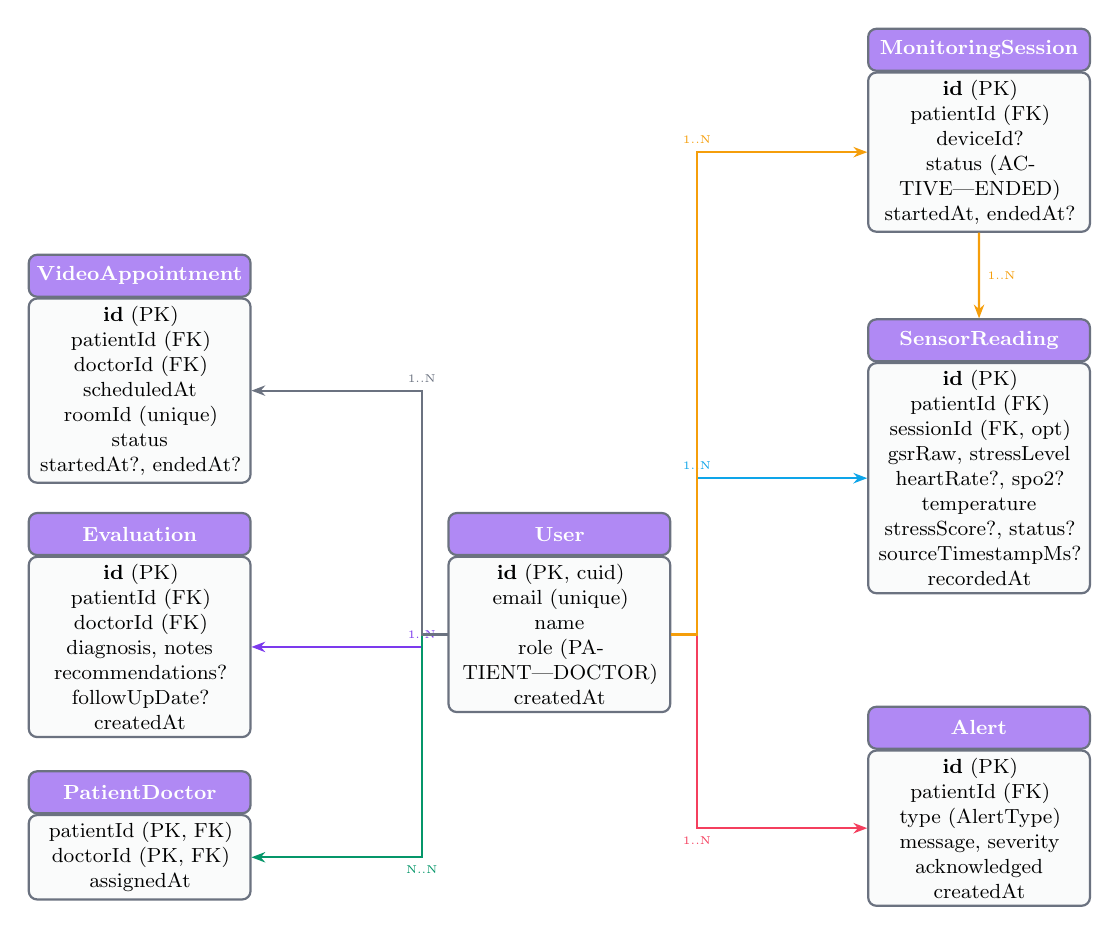
\begin{tikzpicture}[
  node distance=0.3cm,scale=0.82,transform shape,
  tbl/.style={rectangle,draw=midgray,thick,rounded corners=3pt,
    fill=lightgray!40,text width=3.2cm,align=center,font=\small},
  hd/.style={rectangle,draw=midgray,thick,rounded corners=3pt,
    fill=primary!60,text=white,text width=3.2cm,minimum height=0.65cm,
    align=center,font=\small\bfseries},
  rel/.style={arr,midgray,thick},
]

% USER (centre)
\node[hd] (Uh) at (0,0) {User};
\node[tbl,below=0pt of Uh] (Ub) {
  \textbf{id} (PK, cuid)\\
  email (unique)\\
  name\\
  role (PATIENT|DOCTOR)\\
  createdAt
};

% SENSOR READING (right-top)
\node[hd] (SRh) at (6.5,3) {SensorReading};
\node[tbl,below=0pt of SRh] (SRb) {
  \textbf{id} (PK)\\
  patientId (FK)\\
  sessionId (FK, opt)\\
  gsrRaw, stressLevel\\
  heartRate?, spo2?\\
  temperature\\
  stressScore?, status?\\
  sourceTimestampMs?\\
  recordedAt
};

% ALERT (right-bottom)
\node[hd] (Ah) at (6.5,-3) {Alert};
\node[tbl,below=0pt of Ah] (Ab) {
  \textbf{id} (PK)\\
  patientId (FK)\\
  type (AlertType)\\
  message, severity\\
  acknowledged\\
  createdAt
};

% EVALUATION (left)
\node[hd] (Eh) at (-6.5,0) {Evaluation};
\node[tbl,below=0pt of Eh] (Eb) {
  \textbf{id} (PK)\\
  patientId (FK)\\
  doctorId (FK)\\
  diagnosis, notes\\
  recommendations?\\
  followUpDate?\\
  createdAt
};

% PATIENT-DOCTOR (left-bottom)
\node[hd] (PDh) at (-6.5,-4) {PatientDoctor};
\node[tbl,below=0pt of PDh] (PDb) {
  patientId (PK, FK)\\
  doctorId (PK, FK)\\
  assignedAt
};

% MONITORING SESSION (right-top-2)
\node[hd] (MSh) at (6.5,7.5) {MonitoringSession};
\node[tbl,below=0pt of MSh] (MSb) {
  \textbf{id} (PK)\\
  patientId (FK)\\
  deviceId?\\
  status (ACTIVE|ENDED)\\
  startedAt, endedAt?
};

% VIDEO APPOINTMENT (left-top)
\node[hd] (VAh) at (-6.5,4) {VideoAppointment};
\node[tbl,below=0pt of VAh] (VAb) {
  \textbf{id} (PK)\\
  patientId (FK)\\
  doctorId (FK)\\
  scheduledAt\\
  roomId (unique)\\
  status\\
  startedAt?, endedAt?
};

% Relations
\draw[rel,secondary] (Ub.east) -- ++(0.4,0) |- (SRb.west) node[midway,above,font=\tiny]{1..N};
\draw[rel,accent]    (Ub.east) -- ++(0.4,0) |- (Ab.west) node[midway,below,font=\tiny]{1..N};
\draw[rel,primary]   (Ub.west) -- ++(-0.4,0) |- (Eb.east) node[midway,above,font=\tiny]{1..N};
\draw[rel,success]   (Ub.west) -- ++(-0.4,0) |- (PDb.east) node[midway,below,font=\tiny]{N..N};
\draw[rel,codeyellow](Ub.east) -- ++(0.4,0) |- (MSb.west) node[midway,above,font=\tiny]{1..N};
\draw[rel,midgray]   (Ub.west) -- ++(-0.4,0) |- (VAb.east) node[midway,above,font=\tiny]{1..N};
\draw[rel,codeyellow](MSb.south) -- (SRh.north) node[midway,right,font=\tiny]{1..N};
\end{tikzpicture}
\caption{Entity Relationship Diagram --- all Prisma models and relations}
\end{figure}

\section{Model Summary}

\begin{table}[H]\centering\renewcommand{\arraystretch}{1.5}
\begin{tabularx}{\linewidth}{>{\bfseries}l X}
\toprule
Model & Purpose \\
\midrule
User & Central entity. id matches Supabase Auth UID. Role: PATIENT, DOCTOR, ADMIN. \\
SensorReading & Every raw physiological sample from hardware. Indexed on [patientId, recordedAt] and [sessionId, recordedAt]. \texttt{sourceTimestampMs} (BigInt) is the deduplication key. \\
Alert & Auto-generated anomaly. Severity 1--3. Doctor acknowledges to dismiss. \\
Evaluation & Doctor's clinical assessment of a patient. Contains diagnosis, notes, recommendations, optional follow-up date. \\
PatientDoctor & Many-to-many junction. Composite PK [patientId, doctorId]. Auto-populated on registration. \\
MonitoringSession & A discrete monitoring window grouping related SensorReadings. Indexed on [patientId, status] for active session lookup. \\
VideoAppointment & Telemedicine call record. \texttt{roomId} maps to ZegoCloud room. Lifecycle: SCHEDULED $\to$ ACTIVE $\to$ COMPLETED/CANCELLED. \\
\bottomrule
\end{tabularx}
\caption{Prisma model descriptions}
\end{table}

% ============================================================
\chapter{Firebase Integration and Real-Time Sync}

\section{Why Firebase?}

PostgreSQL is not designed for sub-second publish/subscribe. Firebase Realtime Database (RTDB) provides a \textbf{WebSocket channel} that pushes sensor readings to connected browsers in under 100ms. PostgreSQL then serves as the durable store for historical queries.

\begin{figure}[H]\centering
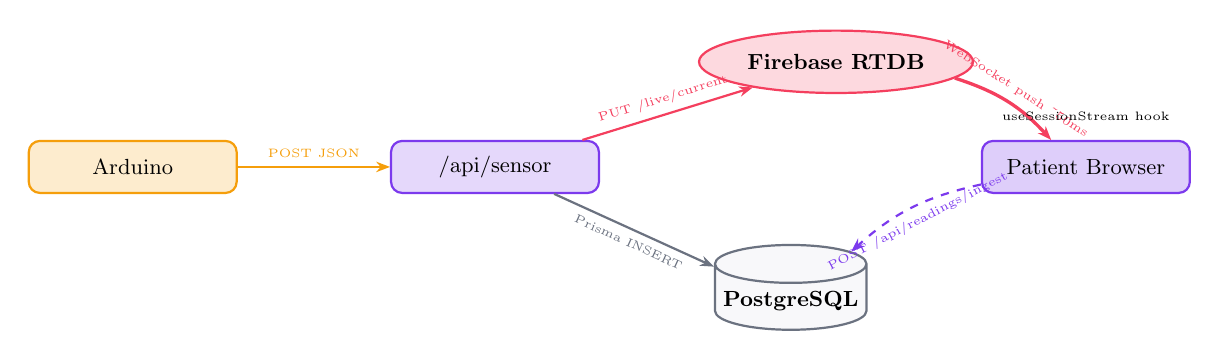
\begin{tikzpicture}[node distance=1.6cm,scale=0.88,transform shape,
  b/.style={box,minimum width=3cm,font=\small}]

\node[b,fill=codeyellow!20,draw=codeyellow] (hw) {Arduino};
\node[b,fill=primary!20,draw=primary,right=2.2cm of hw] (api) {/api/sensor};
\node[cbox,fill=accent!20,draw=accent,above right=0.8cm and 2cm of api] (fb) {Firebase RTDB};
\node[dbox,below right=0.8cm and 2cm of api] (pg) {PostgreSQL};
\node[b,fill=primary!25,draw=primary,right=5.5cm of api] (br) {Patient Browser};

\draw[arr,codeyellow] (hw) -- node[above,font=\tiny]{POST JSON} (api);
\draw[arr,accent] (api) -- node[above,font=\tiny,sloped]{PUT /live/current} (fb);
\draw[arr,midgray] (api) -- node[below,font=\tiny,sloped]{Prisma INSERT} (pg);
\draw[arr,accent,very thick] (fb) to[bend left=15]
  node[above,font=\tiny,sloped]{WebSocket push \textasciitilde{}50ms} (br);
\draw[arr,primary,dashed] (br) to[bend right=15]
  node[below,font=\tiny,sloped]{POST /api/readings/ingest} (pg);
\node[font=\tiny,above=0.15cm of br]{useSessionStream hook};
\end{tikzpicture}
\caption{Dual-write strategy: Firebase for live stream, PostgreSQL for persistence}
\end{figure}

\section{Firebase RTDB Data Structure}

\begin{table}[H]\centering\renewcommand{\arraystretch}{1.4}
\begin{tabularx}{\linewidth}{>{\ttfamily\small}l X}
\toprule
RTDB Path & Purpose \\
\midrule
/live/current/\{sessionId\} & Most recent reading per session (PUT = overwrite). Browser subscribes here for live display. \\
/history/readings/\{sessionId\}/\{pushKey\} & Append-only log of all readings. Synced into PostgreSQL on demand. \\
/bridge/activeSession & Active session metadata. Hardware reads this to know which patient/session to tag readings with. \\
\bottomrule
\end{tabularx}
\caption{Firebase RTDB path reference}
\end{table}

\section{Server-Side Firebase REST API}

The Next.js server cannot use the Firebase SDK (which needs browser WebSockets). All server $\to$ Firebase communication uses the \textbf{Firebase REST API} via \texttt{fetch()}:

\begin{lstlisting}[language=TypeScript,caption={src/lib/firebaseRtdbServer.ts}]
const URL = "https://mindmonitor-2c5f1-default-rtdb.asia-southeast1.firebasedatabase.app";
export const rtdbGet    = (p: string) => fetch(`${URL}/${p}.json`).then(r=>r.json());
export const rtdbPut    = (p: string, d: unknown) =>
  fetch(`${URL}/${p}.json`, { method:"PUT",  body:JSON.stringify(d) });
export const rtdbPost   = (p: string, d: unknown) =>
  fetch(`${URL}/${p}.json`, { method:"POST", body:JSON.stringify(d) });
export const rtdbDelete = (p: string) => fetch(`${URL}/${p}.json`, { method:"DELETE" });
\end{lstlisting}

\section{Deduplication Strategy}

IoT sensors reconnect frequently, causing duplicate readings. The sync layer (\texttt{src/lib/firebaseReadingsSync.ts}) prevents duplicates entering PostgreSQL:

\begin{enumerate}[leftmargin=2em]
  \item \textbf{Primary key:} \texttt{(sessionId, sourceTimestampMs)} --- the ESP8266's own uptime/Unix timestamp.
  \item \textbf{Fallback hash:} If \texttt{sourceTimestampMs} is absent, compare \texttt{(recordedAt $\pm$1s, gsrRaw, temperature, heartRate)} to detect near-duplicates within a 1-second window.
  \item \textbf{Upsert:} Prisma \texttt{upsert} with these keys ensures idempotent writes.
\end{enumerate}

\section{useSessionStream Hook}

\textbf{File:} \texttt{src/hooks/useSessionStream.ts} --- subscribes to Firebase and persists to PostgreSQL.

\begin{lstlisting}[language=TypeScript,caption={Hook interface}]
const { reading, streamStatus, readingCount } = useSessionStream(sessionId);
// reading:      latest RawFirebaseReading | null
// streamStatus: "connecting" | "live" | "disconnected"
// readingCount: total readings this session
\end{lstlisting}

Internally: subscribes via \texttt{onValue(ref(database,\textasciigrave/live/current/\${sid}\textasciigrave))}, updates React state immediately, then calls \texttt{POST /api/readings/ingest} in the background for PostgreSQL persistence. Unsubscribes via \texttt{off()} on unmount.

% ============================================================
\chapter{API Routes}

\begin{table}[H]\centering\renewcommand{\arraystretch}{1.35}
\begin{tabularx}{\linewidth}{>{\ttfamily\small}l >{\small}l X}
\toprule
\textbf{Route} & \textbf{Method} & \textbf{Description} \\
\midrule
\multicolumn{3}{l}{\textbf{Authentication}} \\
/api/auth/register & POST & Create Prisma User after Supabase signup. Auto-assigns patient$\leftrightarrow$doctor. \\
/api/auth/confirm-email & POST & Admin: confirm email without link click (uses service-role key). \\
\midrule
\multicolumn{3}{l}{\textbf{Sensor \& Readings}} \\
/api/sensor & POST & Hardware webhook. Auth: X-API-Key. Writes PostgreSQL + Firebase, triggers anomaly check. \\
/api/readings/ingest & POST & Firebase$\to$PostgreSQL bridge (called by useSessionStream). Deduplicates before INSERT. \\
/api/readings & GET & Fetch readings (?patientId, ?range=24h|7d|30d). Auto-syncs Firebase history. \\
\midrule
\multicolumn{3}{l}{\textbf{Sessions}} \\
/api/sessions & GET & Get active session for patient (?patientId). \\
/api/sessions & POST & Create monitoring session (ends any existing active session first). \\
/api/sessions/[id]/end & PATCH & Set session status to ENDED, record endedAt. \\
/api/sessions/[id]/stream & GET & SSE stream of synthetic sensor data (demo mode). \\
\midrule
\multicolumn{3}{l}{\textbf{Alerts}} \\
/api/alerts & GET & List alerts (?doctorId or ?patientId, ?acknowledged=true|false). \\
/api/alerts & POST & Create alert manually. \\
/api/alerts/[id]/acknowledge & PATCH & Set acknowledged=true. \\
\midrule
\multicolumn{3}{l}{\textbf{Patients}} \\
/api/patients & GET & Doctor's assigned patients with latest reading + alert count (?doctorId). \\
/api/patients/available & GET & Patients not yet assigned to a doctor (?doctorId). \\
/api/patients/assign & POST & Assign patient to doctor (upsert). \\
\midrule
\multicolumn{3}{l}{\textbf{Appointments}} \\
/api/appointments & GET & List appointments (?patientId or ?doctorId, ?status). \\
/api/appointments & POST & Schedule appointment. Creates VideoAppointment with auto-generated roomId. \\
/api/appointments/[id] & PATCH & Update status (sets startedAt or endedAt). \\
/api/appointments/[id] & DELETE & Delete appointment. \\
\midrule
\multicolumn{3}{l}{\textbf{Evaluations}} \\
/api/evaluations & GET & List evaluations (?patientId), newest first. \\
/api/evaluations & POST & Create evaluation. Zod-validated body: \{patientId, doctorId, diagnosis, notes, recommendations?, followUpDate?\}. \\
\bottomrule
\end{tabularx}
\caption{All API endpoints}
\end{table}

% ============================================================
\chapter{Video Call System}

\section{ZegoCloud Integration}

Video consultations use \textbf{ZegoCloud UIKit Prebuilt}, a WebRTC wrapper that provides a complete video call UI without manual signalling server setup.

\begin{lstlisting}[language=JavaScript,caption={ZegoCloud room join pattern (from ZEGO.md)}]
const kitToken = ZegoUIKitPrebuilt.generateKitTokenForTest(
  appID,        // 2015575164
  serverSecret, // from env
  roomID,       // VideoAppointment.roomId (cuid)
  userId, userName
);
const zp = ZegoUIKitPrebuilt.create(kitToken);
zp.joinRoom({ container: element,
  scenario: { mode: ZegoUIKitPrebuilt.OneONoneCall } });
\end{lstlisting}

\section{Appointment Flow}

\begin{enumerate}[leftmargin=2em]
  \item Doctor calls \texttt{POST /api/appointments} $\to$ creates \texttt{VideoAppointment} row with unique \texttt{roomId} (cuid).
  \item Both patient and doctor see the appointment in their dashboards (\texttt{GET /api/appointments}).
  \item At call time: \texttt{PATCH /api/appointments/[id]} sets \texttt{status=ACTIVE}, records \texttt{startedAt}.
  \item Frontend generates a ZegoCloud kit token using the \texttt{roomId} and joins the room.
  \item On end: \texttt{PATCH} sets \texttt{status=COMPLETED}, records \texttt{endedAt}.
\end{enumerate}

\begin{dangerbox}[Critical Security Issue: Server Secret Exposed]
\texttt{NEXT\_PUBLIC\_ZEGO\_SERVER\_SECRET} is embedded in the browser JavaScript bundle (any \texttt{NEXT\_PUBLIC\_} var is public). Any user can read it from DevTools and mint tokens for any ZegoCloud room.

\textbf{Fix:} Add a \texttt{POST /api/appointments/[id]/token} route that generates the token server-side and returns only the short-lived token string to the browser.
\end{dangerbox}

% ============================================================
\chapter{Anomaly Detection and Alerts}

\section{Rule-Based Engine}

\textbf{File:} \texttt{src/lib/anomaly.ts}

Every new \texttt{SensorReading} insertion triggers a rule evaluation. No machine learning --- purely threshold-based:

\begin{table}[H]\centering\renewcommand{\arraystretch}{1.5}
\begin{tabularx}{\linewidth}{l c X}
\toprule
\textbf{Alert Type} & \textbf{Severity} & \textbf{Trigger} \\
\midrule
HIGH\_STRESS & 3 (Critical) & \texttt{stressLevel = 3} on current reading \\
PROLONGED\_STRESS & 2 (Warning) & Last 5+ consecutive readings all have \texttt{stressLevel $\geq$ 2} \\
TEMPERATURE\_ANOMALY & 2 (Warning) & \texttt{temperature < 35.5\textdegree{}C} or \texttt{> 37.8\textdegree{}C} \\
RAPID\_CHANGE & --- & Defined in enum, not yet triggered by current rules \\
\bottomrule
\end{tabularx}
\caption{Anomaly detection rules}
\end{table}

\section{Alert Lifecycle}

New reading $\to$ Anomaly engine $\to$ \texttt{Alert} row in PostgreSQL $\to$ Badge on doctor dashboard $\to$ Doctor acknowledges $\to$ \texttt{acknowledged = true} $\to$ Removed from unacknowledged feed.

% ============================================================
\chapter{Frontend Architecture}

\section{Next.js App Router Structure}

\begin{table}[H]\centering\renewcommand{\arraystretch}{1.4}
\begin{tabularx}{\linewidth}{>{\ttfamily\small}l l X}
\toprule
URL & Access & Content \\
\midrule
/ & Public & Landing page (Hero, Problem, Solution, Features) \\
/login & Public & Supabase sign-in form \\
/register & Public & Sign-up with role selector + password strength meter \\
/doctor/dashboard & DOCTOR & Patient list, alert summary, quick stats per patient \\
/doctor/dashboard/evaluate & DOCTOR & Clinical evaluation form \\
/doctor/dashboard/patients/[id] & DOCTOR & Full patient detail (charts, evaluations, appointments) \\
/patient/dashboard & PATIENT & Live monitoring + all charts + readings table \\
/patient/dashboard/evaluations & PATIENT & All received evaluations \\
/patient/dashboard/history & PATIENT & Historical readings with time-range filter \\
\bottomrule
\end{tabularx}
\caption{Page routes and roles}
\end{table}

Pages are \textbf{Server Components} by default (data fetched server-side). Interactive parts are \textbf{Client Components} (\texttt{"use client"}) for real-time state and event handling.

\section{Key Components}

\begin{table}[H]\centering\renewcommand{\arraystretch}{1.4}
\begin{tabularx}{\linewidth}{>{\bfseries\small}l X}
\toprule
Component & Role \\
\midrule
MonitoringPanel & Start/stop sessions, display real-time vitals. Uses \texttt{useSessionStream} hook. \\
LiveReadingCards & 5 cards: heart rate, SpO2, GSR, GSR delta, temperature. \\
StressLineChart & Recharts line chart of stress level over time. \\
StressDistributionPie & Pie chart of normal / elevated / high stress distribution. \\
TemperatureGauge & Gauge visualization of current temperature. \\
VitalsLineChart & Heart rate and SpO2 trend lines. \\
GsrLineChart & Raw GSR and delta (gsrDiff) trends. \\
PatientListSidebar & Doctor's patient list sorted by alert count $\times$ stress level. \\
PatientDetailPanel & Doctor: charts + history + evaluations for one patient. \\
AlertFeed & List of unacknowledged alerts with acknowledge button. \\
EvaluationForm & Zod-validated form to create clinical evaluations. \\
AppointmentScheduler & Schedule video appointments (calls POST /api/appointments). \\
Navbar & Sticky nav with role badge, live indicator, logout. \\
\bottomrule
\end{tabularx}
\caption{Key UI components and their purpose}
\end{table}

\section{State Management}

No external state library (Redux, Zustand) is used. Plain React patterns suffice:

\begin{description}[leftmargin=3cm,labelwidth=2.5cm]
  \item[\texttt{useState}] Form values, UI toggles, loading flags, current readings.
  \item[\texttt{useEffect}] API calls on mount, Firebase subscriptions, auth state listeners.
  \item[\texttt{useRef}] Firebase listener handles (for \texttt{off()} cleanup), interval IDs.
  \item[\texttt{useCallback}] Stable function references passed to child components.
  \item[Props] Server Components fetch data and pass it down to Client Components.
\end{description}

\section{Design System}

Dark glassmorphism theme matching the landing page throughout:

\begin{itemize}[leftmargin=2em]
  \item \textbf{Background:} \texttt{bg-gray-950} (\#030712)
  \item \textbf{Cards:} \texttt{bg-white/5 backdrop-blur-md border border-white/10}
  \item \textbf{Accent:} Violet gradient (\texttt{from-violet-600 to-violet-500})
  \item \textbf{Status colors:} Green (normal), Orange (elevated), Red (high stress)
  \item \textbf{Animation:} Framer Motion fade-in, slide-up, hover scale
\end{itemize}

% ============================================================
\chapter{End-to-End Data Flows}

\section{Live Sensor Reading Flow}

\begin{figure}[H]\centering
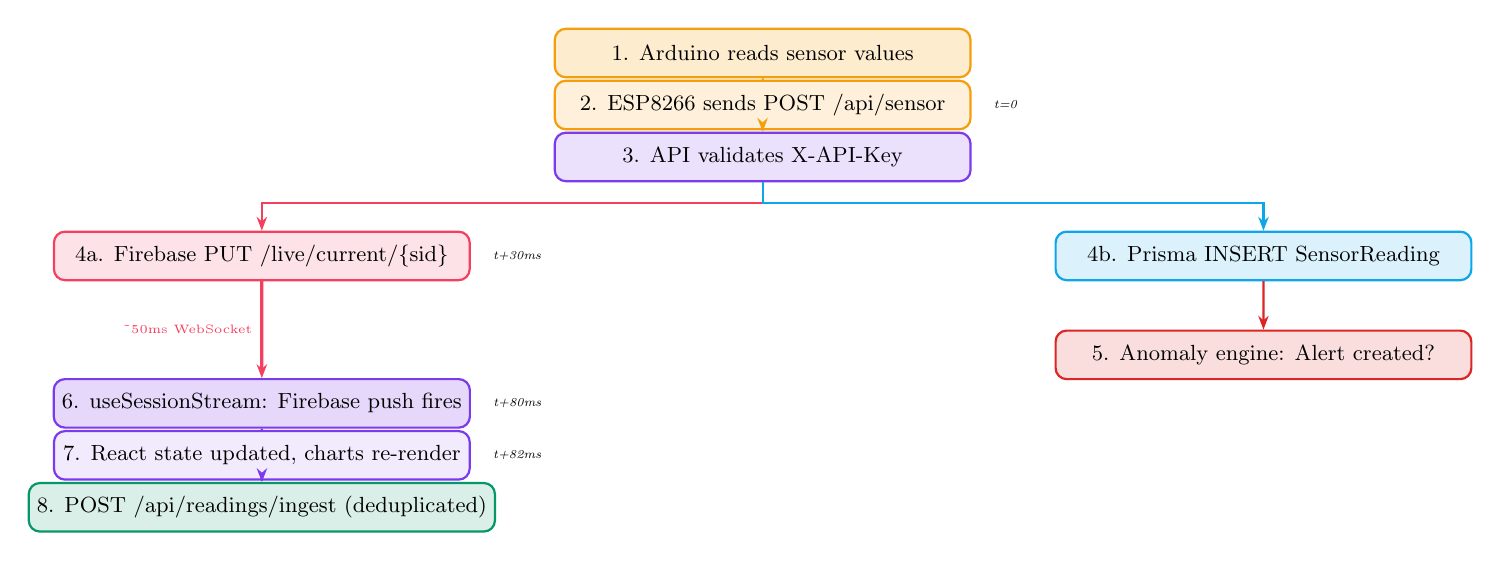
\begin{tikzpicture}[node distance=0.75cm,scale=0.88,transform shape,
  s/.style={box,minimum width=6cm,minimum height=0.7cm,font=\small}]

\node[s,fill=codeyellow!20,draw=codeyellow] (s0) {1. Arduino reads sensor values};
\node[s,fill=codeyellow!15,draw=codeyellow,below of=s0] (s1) {2. ESP8266 sends POST /api/sensor};
\node[s,fill=primary!15,draw=primary,below of=s1] (s2) {3. API validates X-API-Key};

\node[s,fill=accent!15,draw=accent,below left=0.7cm and 1.2cm of s2] (fb)
  {4a. Firebase PUT /live/current/\{sid\}};
\node[s,fill=secondary!15,draw=secondary,below right=0.7cm and 1.2cm of s2] (pg)
  {4b. Prisma INSERT SensorReading};

\node[s,fill=danger!15,draw=danger,below=0.7cm of pg] (an)
  {5. Anomaly engine: Alert created?};
\node[s,fill=primary!20,draw=primary,below=1.4cm of fb] (hook)
  {6. useSessionStream: Firebase push fires};
\node[s,fill=primary!10,draw=primary,below of=hook] (ui)
  {7. React state updated, charts re-render};
\node[s,fill=success!15,draw=success,below of=ui] (ing)
  {8. POST /api/readings/ingest (deduplicated)};

\draw[arr,codeyellow] (s0)--(s1)--(s2);
\draw[arr,accent] (s2.south) -- ++(0,-0.3) -| (fb.north);
\draw[arr,secondary] (s2.south) -- ++(0,-0.3) -| (pg.north);
\draw[arr,danger] (pg)--(an);
\draw[arr,accent,very thick] (fb.south) -- node[left,font=\tiny]{\textasciitilde{}50ms WebSocket} (hook.north);
\draw[arr,primary] (hook)--(ui)--(ing);

\node[font=\tiny\itshape,right=0.2cm of s1] {t=0};
\node[font=\tiny\itshape,right=0.2cm of fb] {t+30ms};
\node[font=\tiny\itshape,right=0.2cm of hook] {t+80ms};
\node[font=\tiny\itshape,right=0.2cm of ui] {t+82ms};
\end{tikzpicture}
\caption{Complete data flow for one sensor reading, from hardware to browser UI}
\end{figure}

% ============================================================
\chapter{Security Analysis}

\begin{table}[H]\centering\renewcommand{\arraystretch}{1.5}
\begin{tabularx}{\linewidth}{>{\bfseries}l X >{\bfseries}l}
\toprule
Control & Status & Rating \\
\midrule
JWT in HTTP-only cookies & Supabase SSR auto-manages cookie storage & \textcolor{success}{Good} \\
JWT validation & Signature + expiry checked on every request & \textcolor{success}{Good} \\
Route protection & Middleware guards all protected paths & \textcolor{success}{Good} \\
Role-based access & Doctor / Patient routes reject wrong roles & \textcolor{success}{Good} \\
Hardware auth & X-API-Key header on /api/sensor & \textcolor{success}{Good} \\
Admin client & service-role key server-side only & \textcolor{success}{Good} \\
\midrule
ZegoCloud server secret & NEXT\_PUBLIC\_ exposes it in browser bundle & \textcolor{danger}{Critical} \\
Firebase RTDB rules & Database in test mode --- no auth required & \textcolor{warning}{High} \\
API route auth & Most routes have no authentication check & \textcolor{warning}{High} \\
Input validation & Zod only on /api/evaluations POST & \textcolor{warning}{Medium} \\
Rate limiting & No rate limiting on any endpoint & \textcolor{warning}{Medium} \\
Email confirm bypass & /api/auth/confirm-email unprotected & \textcolor{warning}{Medium} \\
\bottomrule
\end{tabularx}
\caption{Security audit summary}
\end{table}

\begin{dangerbox}[Top Priorities to Fix]
\begin{enumerate}[leftmargin=2em]
  \item Move ZegoCloud token generation server-side. Remove \texttt{NEXT\_PUBLIC\_ZEGO\_SERVER\_SECRET}.
  \item Add Firebase Security Rules to restrict RTDB reads/writes.
  \item Add Supabase JWT validation to all API routes (create a shared \texttt{requireAuth()} helper).
\end{enumerate}
\end{dangerbox}

% ============================================================
\chapter{Deployment and Environment}

\section{Environment Variables}

\begin{table}[H]\centering\renewcommand{\arraystretch}{1.4}
\begin{tabularx}{\linewidth}{>{\ttfamily\small}l l X}
\toprule
Variable & Visibility & Purpose \\
\midrule
NEXT\_PUBLIC\_SUPABASE\_URL & Public & Supabase project URL \\
NEXT\_PUBLIC\_SUPABASE\_ANON\_KEY & Public & Supabase anonymous key \\
SUPABASE\_SERVICE\_ROLE\_KEY & Server-only & Admin operations \\
DATABASE\_URL & Server-only & Prisma runtime (pooled port 6543) \\
DIRECT\_URL & Server-only & Prisma migrations (direct port 5432) \\
ARDUINO\_API\_KEY & Server-only & Shared secret for /api/sensor \\
NEXT\_PUBLIC\_ZEGO\_APP\_ID & Public & ZegoCloud App ID \\
NEXT\_PUBLIC\_ZEGO\_SERVER\_SECRET & \textcolor{danger}{Exposed} & Should be server-only \\
\bottomrule
\end{tabularx}
\caption{Environment variables}
\end{table}

\section{Commands}

\begin{lstlisting}[language=bash,caption={Development and production commands}]
npm install                   # Install dependencies
npx prisma generate           # Generate Prisma client
npx prisma db push            # Push schema to DB (dev)
npx prisma migrate deploy     # Apply migrations (prod)
npm run dev                   # Development server
npm run build && npm start    # Production build + run
npx prisma studio             # GUI database browser
\end{lstlisting}

% ============================================================
\chapter{Glossary}

\begin{description}[leftmargin=3cm,labelwidth=2.8cm,style=nextline]
  \item[App Router] Next.js 13+ routing using the \texttt{src/app/} directory.
  \item[CUID] Collision-resistant Unique ID --- URL-safe, lexicographically sortable.
  \item[Firebase RTDB] Firebase Realtime Database --- JSON tree synced via WebSocket.
  \item[GSR] Galvanic Skin Response --- skin conductance rises with emotional arousal.
  \item[JWT] JSON Web Token --- signed, self-contained token carrying user claims.
  \item[ORM] Object-Relational Mapper --- type-safe language-layer over SQL.
  \item[PgBouncer] PostgreSQL connection pooler on port 6543 (Supabase).
  \item[Prisma] TypeScript ORM: schema + auto-generated client + migrate CLI.
  \item[SpO\textsubscript{2}] Peripheral capillary oxygen saturation (pulse oximetry).
  \item[SSE] Server-Sent Events --- one-way HTTP streaming from server to browser.
  \item[SSR] Server-Side Rendering --- HTML generated on server per request.
  \item[Supabase] Open-source Firebase alternative on PostgreSQL (Auth + DB + Storage).
  \item[WebRTC] Browser API for peer-to-peer audio/video.
  \item[ZegoCloud] Cloud WebRTC platform with prebuilt video call UI kits.
\end{description}

% ============================================================
\appendix
\chapter{Full Prisma Schema}

\begin{lstlisting}[language=TypeScript,caption={prisma/schema.prisma}]
generator client {
  provider = "prisma-client-js"
  output   = "./src/generated/prisma"
}
datasource db {
  provider  = "postgresql"
  url       = env("DATABASE_URL")
  directUrl = env("DIRECT_URL")
}

enum Role             { PATIENT DOCTOR ADMIN }
enum AlertType        { HIGH_STRESS PROLONGED_STRESS RAPID_CHANGE TEMPERATURE_ANOMALY }
enum SessionStatus    { ACTIVE ENDED }
enum AppointmentStatus{ SCHEDULED ACTIVE COMPLETED CANCELLED }

model User {
  id        String   @id @default(cuid())
  email     String   @unique
  name      String
  role      Role     @default(PATIENT)
  createdAt DateTime @default(now())
  readings              SensorReading[]    @relation("PatientReadings")
  alerts                Alert[]            @relation("PatientAlerts")
  evaluationsReceived   Evaluation[]       @relation("PatientEvaluations")
  evaluationsGiven      Evaluation[]       @relation("DoctorEvaluations")
  assignedPatients      PatientDoctor[]    @relation("DoctorAssignments")
  assignedDoctors       PatientDoctor[]    @relation("PatientAssignments")
  monitoringSessions    MonitoringSession[]
  appointmentsAsPatient VideoAppointment[] @relation("PatientAppointments")
  appointmentsAsDoctor  VideoAppointment[] @relation("DoctorAppointments")
}

model SensorReading {
  id          String   @id @default(cuid())
  patientId   String
  sessionId   String?
  deviceId    String?
  gsrRaw      Int
  stressLevel Int
  stressLabel String
  heartRate   Int?
  spo2        Float?
  temperature Float
  gsrBaseline      Int?
  gsrDiff          Int?
  ir               Int?
  red              Int?
  fingerDetected   Boolean?
  skinDetected     Boolean?
  stressScore      Int?
  status           String?
  sourceTimestampMs BigInt?
  recordedAt  DateTime @default(now())
  patient User              @relation("PatientReadings", fields:[patientId], references:[id])
  session MonitoringSession? @relation(fields:[sessionId], references:[id])
  @@index([patientId, recordedAt])
  @@index([sessionId, recordedAt])
}

model Alert {
  id           String    @id @default(cuid())
  patientId    String
  type         AlertType
  message      String
  severity     Int
  acknowledged Boolean   @default(false)
  createdAt    DateTime  @default(now())
  patient      User      @relation("PatientAlerts", fields:[patientId], references:[id])
}

model Evaluation {
  id              String    @id @default(cuid())
  patientId       String
  doctorId        String
  diagnosis       String
  notes           String
  recommendations String?
  followUpDate    DateTime?
  createdAt       DateTime  @default(now())
  patient User @relation("PatientEvaluations", fields:[patientId], references:[id])
  doctor  User @relation("DoctorEvaluations",  fields:[doctorId],  references:[id])
}

model PatientDoctor {
  patientId  String
  doctorId   String
  assignedAt DateTime @default(now())
  patient User @relation("PatientAssignments", fields:[patientId], references:[id])
  doctor  User @relation("DoctorAssignments",  fields:[doctorId],  references:[id])
  @@id([patientId, doctorId])
}

model MonitoringSession {
  id        String        @id @default(cuid())
  patientId String
  deviceId  String?
  status    SessionStatus @default(ACTIVE)
  startedAt DateTime      @default(now())
  endedAt   DateTime?
  patient  User            @relation(fields:[patientId], references:[id])
  readings SensorReading[]
  @@index([patientId, status])
}

model VideoAppointment {
  id          String            @id @default(cuid())
  patientId   String
  doctorId    String
  scheduledAt DateTime
  roomId      String            @unique @default(cuid())
  status      AppointmentStatus @default(SCHEDULED)
  startedAt   DateTime?
  endedAt     DateTime?
  createdAt   DateTime          @default(now())
  patient User @relation("PatientAppointments", fields:[patientId], references:[id])
  doctor  User @relation("DoctorAppointments",  fields:[doctorId],  references:[id])
  @@index([patientId])
  @@index([doctorId])
}
\end{lstlisting}

\end{document}
